\input{preamble.tex}
\newcommand{\C}{\mathcal{C}}
\pgfplotsset{tick style={very thin}} 


\begin{document}
\pagestyle{fancy}
\fancyhead[L]{Seconde}
\fancyhead[C]{\textbf{Evaluation flash n°3a}}
\fancyhead[R]{\today}

\reversemarginpar

\null\vspace{-30pt}
Nom / Prénom : \\

Consignes particulières : 
\begin{itemize}[label=$\bullet$]
	\item 
	La calculatrice est \textbf{interdite}.
%	\item 
%	Le devoir peut être fait entièrement sur cette feuille.
%	\item 
%	Toute trace de recherche est prise en compte.
	%\item 
	%L'abbréviation $\tq$ signifie ``tel que''.
\end{itemize}

\hrule

\exe{4}{
On donne $f(x) = \dfrac32 x - 2$. 
\begin{enumerate}
\item Donner les paramètres $a$ et $b$ de la fonction affine $f$. 
\item Représenter $\C_f$ dans un repère orthonormé.
\item Le point $P \left ( \dfrac23 ; -1 \right )$ appartient-il à $\C_f$ ? Justifier.
\item Donner l'expression algébrique d'une fonction $g$ telle que les droites $\C_g$ et $\C_f$ soient parallèles et telle que
le point $Q \left ( 1 ; 2 \right )$ appartienne à $\C_g$.
\end{enumerate}
}{exe:1a}{
\begin{enumerate}
\item $a=\dfrac32$ et $b=-2$.
\item 
	\begin{center}
	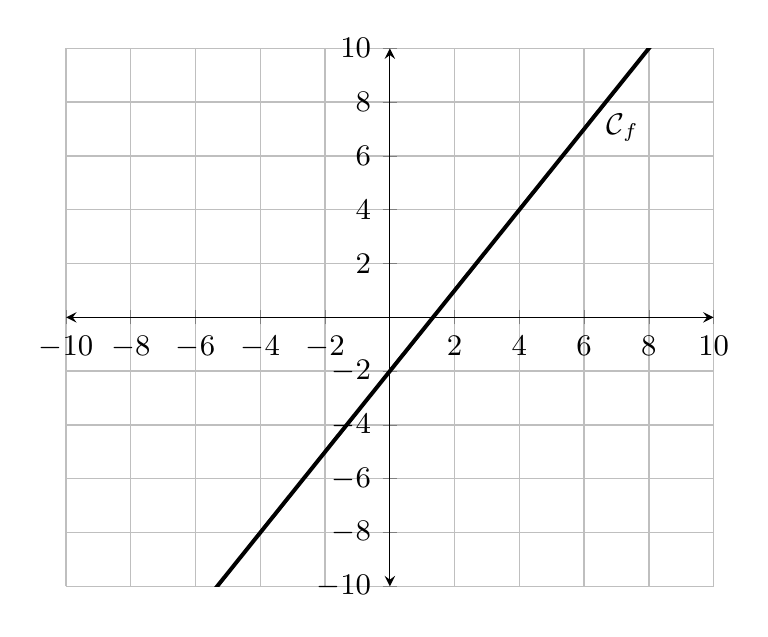
\begin{tikzpicture}[>=stealth, scale=1.2, every node/.append style={font=\small}]
	\begin{axis}[xmin = -10, xmax=10, ymin=-10, ymax=10, axis x line=middle, axis y line=middle, axis line style=<->, xlabel={}, ylabel={}, xtick = {-10, -8, ..., 8, 10}, ytick = {-10, -8, ..., 8, 10}, grid=both]
	
		\addplot[black, very thick, domain =-9:9, samples=2] {3*x/2-2}  node[pos=.9, below=6pt] {$\mathcal{C}_f$};
		\addplot[black, very thick, dotted, domain =-10:-9, samples=2] {3*x/2-2} ;
		\addplot[black, very thick, dotted, domain =9:10, samples=2] {3*x/2-2} ;
	
	\end{axis}
	\end{tikzpicture}
	\end{center}
\item On teste $f  \left ( \dfrac23 \right ) = \dfrac32 \times \dfrac23 - 2 = 1 - 2 = -1$ donc oui.
\item La condition de parallélisme donne le coefficient directeur, donc $g(x) = \dfrac32x + b$.
Pour déterminer $b$ on résout $g(1) = 2$ soit $\dfrac32 + b = 2$ ce qui donne $b=\dfrac12$.
\end{enumerate}
}

\exe{6}{
On considère les deux droites $\C_f$ et $\C_g$ représentées dans le repère ci-dessous.
	\begin{center}
	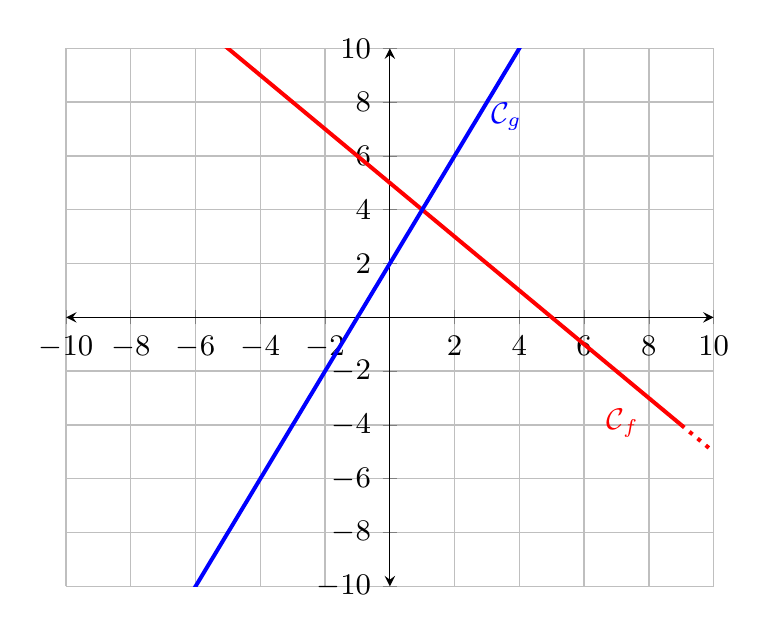
\begin{tikzpicture}[>=stealth, scale=1.2, every node/.append style={font=\small}]
	\begin{axis}[xmin = -10, xmax=10, ymin=-10, ymax=10, axis x line=middle, axis y line=middle, axis line style=<->, xlabel={}, ylabel={}, xtick = {-10, -8, ..., 8, 10}, ytick = {-10, -8, ..., 8, 10}, grid=both]
	
		\addplot[red, very thick, domain =-9:9, samples=2] {-x+5}  node[pos=.9, below=6pt] {$\mathcal{C}_f$};
		\addplot[red, very thick, dotted, domain =-10:-9, samples=2] {-x+5} ;
		\addplot[red, very thick, dotted, domain =9:10, samples=2] {-x+5};
	
	
		\addplot[blue, very thick, domain =-9:9, samples=2] {2*x+2}  node[pos=.7, below=6pt] {$\mathcal{C}_g$};
		\addplot[blue, very thick, dotted, domain =-10:-9, samples=2] {2*x+2} ;
		\addplot[blue, very thick, dotted, domain =9:10, samples=2] {2*x+2};
	\end{axis}
	\end{tikzpicture}
	\end{center}
\begin{enumerate}
\item Pour chacune des droites ci-dessus, donner $2$ points lui appartenant, dont un d'abscisse nulle.
\item Donner les deux ordonnées à l'origine $b$ des fonctions affines associées.
\item Lire graphiquement ou calculer les vecteurs directeurs des deux droites.
\item En déduire les coefficients directeurs $a$ des fonctions affines associées.
\item Ecrire l'expression algébrique des fonctions.
\item Résourdre l'équation $f(x)=g(x)$, en déduire l'abscisse du point $I$ à l'intersection des courbes $\C_f$ et $\C_g$.
\end{enumerate}
}{exe:2a}{
\begin{enumerate}
\item Pour $\C_f$ on a $A(0;5)$ et $B(5;0)$. \\
Pour $\C_g$ on a $C(0;2)$ et $B(2;6)$. \\
\item Respectivement $b=5$ pour $f$ et $b=2$ pour $g$.
\item Pour $f$ : $\vec{AB}=\pvec{5}{-5}$ et pour $g$ : $\vec{CD}=\pvec{2}{4}$
\item On cherche un vecteur colinéaire à $\vec{AB}$ dont la première composante est 1,
soit $\pvec{5}{-5}$ colinéaire à $\pvec{1}{-1}$ et donc $a=-1$ pour $f$. 
En procédant de même, on trouve $a=2$ pour $g$.
\item $f(x) = -x+5$ et $g(x)=2x+2$.
\item $-x+5=2x+2 \iff 3x=3 \iff x=1$.
\end{enumerate}
}

\newpage

\setcounter{Exercise}{0}

\pagestyle{fancy}
\fancyhead[L]{Seconde}
\fancyhead[C]{\textbf{Evaluation flash n°3b}}
\fancyhead[R]{\today}

\reversemarginpar

\null\vspace{-30pt}
Nom / Prénom : \\

Consignes particulières : 
\begin{itemize}[label=$\bullet$]
	\item 
	La calculatrice est \textbf{interdite}.
%	\item 
%	Le devoir peut être fait entièrement sur cette feuille.
%	\item 
%	Toute trace de recherche est prise en compte.
	%\item 
	%L'abbréviation $\tq$ signifie ``tel que''.
\end{itemize}

\hrule

\exe{}{
On donne $f(x) = \dfrac23 x - 3$. 
\begin{enumerate}
\item Donner les paramètres $a$ et $b$ de la fonction affine $f$. 
\item Représenter $\C_f$ dans un repère orthonormé.
\item Le point $P \left ( \dfrac32 ; -2 \right )$ appartient-il à $\C_f$ ? Justifier.
\item Donner l'expression algébrique d'une fonction $g$ telle que les droites $\C_g$ et $\C_f$ soient parallèles et telle que
le point $Q \left ( 1 ; 1 \right )$ appartienne à $\C_g$.
\end{enumerate}
}{exe:1b}{
\begin{enumerate}
\item $a=\dfrac23$ et $b=-3$.
\item 
	\begin{center}
	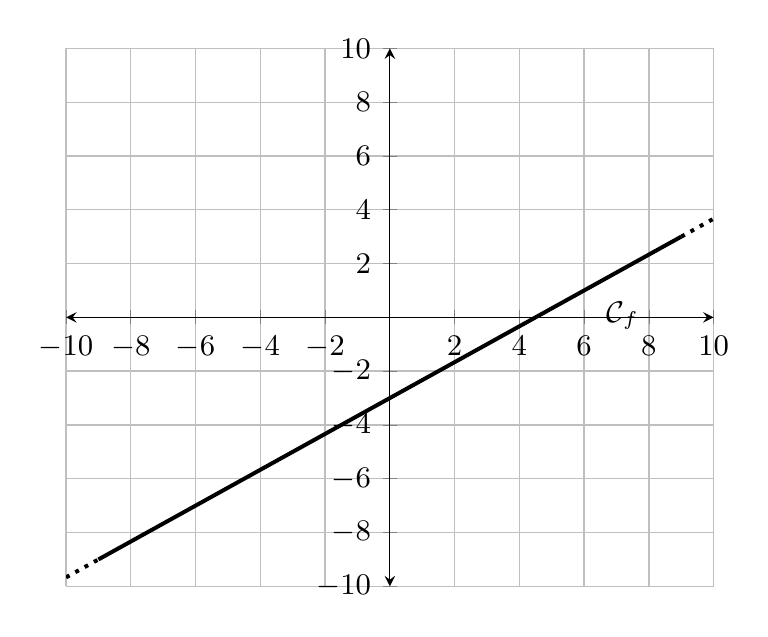
\begin{tikzpicture}[>=stealth, scale=1.2, every node/.append style={font=\small}]
	\begin{axis}[xmin = -10, xmax=10, ymin=-10, ymax=10, axis x line=middle, axis y line=middle, axis line style=<->, xlabel={}, ylabel={}, xtick = {-10, -8, ..., 8, 10}, ytick = {-10, -8, ..., 8, 10}, grid=both]
	
		\addplot[black, very thick, domain =-9:9, samples=2] {2*x/3-3}  node[pos=.9, below=6pt] {$\mathcal{C}_f$};
		\addplot[black, very thick, dotted, domain =-10:-9, samples=2] {2*x/3-3} ;
		\addplot[black, very thick, dotted, domain =9:10, samples=2] {2*x/3-3} ;
	
	\end{axis}
	\end{tikzpicture}
	\end{center}
\item On teste $f  \left ( \dfrac32 \right ) = \dfrac23 \times \dfrac32 - 3 = 1 - 3 = -2$ donc oui.
\item La condition de parallélisme donne le coefficient directeur, donc $g(x) = \dfrac23x + b$.
Pour déterminer $b$ on résout $g(1) = 1$ soit $\dfrac23 + b = 1$ ce qui donne $b=\dfrac13$.
\end{enumerate}
}

\exe{}{
On considère les deux droites $\C_f$ et $\C_g$ représentées dans le repère ci-dessous.
	\begin{center}
	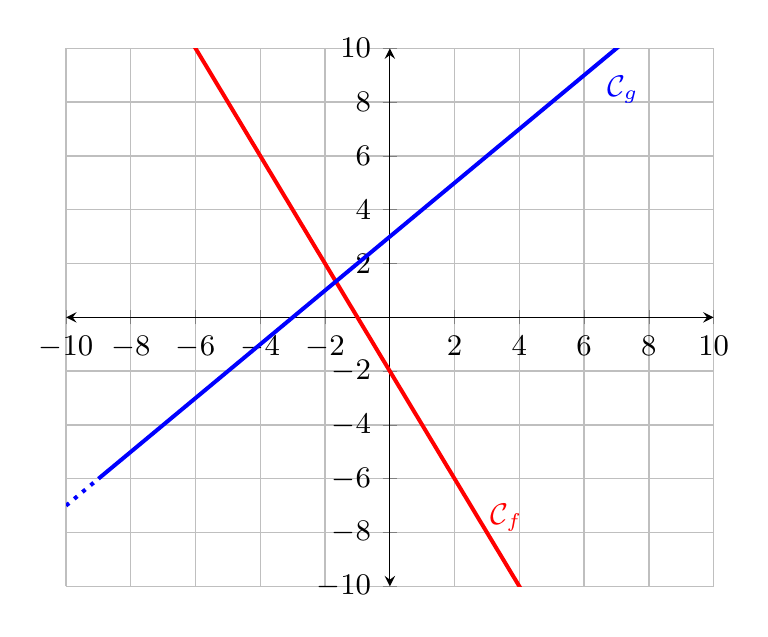
\begin{tikzpicture}[>=stealth, scale=1.2, every node/.append style={font=\small}]
	\begin{axis}[xmin = -10, xmax=10, ymin=-10, ymax=10, axis x line=middle, axis y line=middle, axis line style=<->, xlabel={}, ylabel={}, xtick = {-10, -8, ..., 8, 10}, ytick = {-10, -8, ..., 8, 10}, grid=both]
	
		\addplot[red, very thick, domain =-9:9, samples=2] {-2*x-2}  node[pos=.7, above=6pt] {$\mathcal{C}_f$};
		\addplot[red, very thick, dotted, domain =-10:-9, samples=2] {-2*x-2} ;
		\addplot[red, very thick, dotted, domain =9:10, samples=2] {-2*x-2};
	
	
		\addplot[blue, very thick, domain =-9:9, samples=2] {x+3}  node[pos=.9, below=6pt] {$\mathcal{C}_g$};
		\addplot[blue, very thick, dotted, domain =-10:-9, samples=2] {x+3} ;
		\addplot[blue, very thick, dotted, domain =9:10, samples=2] {x+3};
	\end{axis}
	\end{tikzpicture}
	\end{center}
\begin{enumerate}
\item Pour chacune des droites ci-dessus, donner $2$ points lui appartenant, dont un d'abscisse nulle.
\item Donner les deux ordonnées à l'origine $b$ des fonctions affines associées.
\item Lire graphiquement ou calculer les vecteurs directeurs des deux droites.
\item En déduire les coefficients directeurs $a$ des fonctions affines associées.
\item Ecrire l'expression algébrique des fonctions.
\item Résourdre l'équation $f(x)=g(x)$, en déduire l'abscisse du point $I$ à l'intersection des courbes $\C_f$ et $\C_g$.
\end{enumerate}
}{exe:2b}{
\begin{enumerate}
\item Pour $\C_f$ on a $A(0;-2)$ et $B(2;-6)$. \\
Pour $\C_g$ on a $C(0;3)$ et $B(2;5)$. \\
\item Respectivement $b=-2$ pour $f$ et $b=3$ pour $g$.
\item Pour $f$ : $\vec{AB}=\pvec{2}{-4}$ et pour $g$ : $\vec{CD}=\pvec{2}{2}$
\item On cherche un vecteur colinéaire à $\vec{AB}$ dont la première composante est 1,
soit $\pvec{2}{-4}$ colinéaire à $\pvec{1}{-2}$ et donc $a=-2$ pour $f$. 
En procédant de même, on trouve $a=1$ pour $g$.
\item $f(x) = -2x-2$ et $g(x)=x+3$.
\item $-2x-2=x+3 \iff 3x=-5 \iff x=-\dfrac53$.
\end{enumerate}

}


%%%%%%%%%%%%

\newpage
\fancyhead[C]{\textbf{Solutions}}
\shipoutAnswer

\end{document}
 